\documentclass[12pt]{article}
\usepackage[left=1cm, right=1cm, top=2cm,bottom=1.5cm]{geometry} 

\usepackage[parfill]{parskip}
\usepackage[utf8]{inputenc}
\usepackage[T2A]{fontenc}
\usepackage[russian]{babel}
\usepackage{enumitem}
\usepackage[normalem]{ulem}
\usepackage{amsfonts, amsmath, amsthm, amssymb, mathtools}

\usepackage{fancyhdr}
\pagestyle{fancy}
\renewcommand{\headrulewidth}{1.5pt}
\renewcommand{\footrulewidth}{1pt}

\usepackage{graphicx}
\usepackage[figurename=Рис.]{caption}
\usepackage{subcaption}
\usepackage{float}

%%Наименование папки откуда забирать изображения
\graphicspath{ {./images/} }

%%Изменение формата для ввода доказательства
\renewcommand{\proofname}{$\square$  \nopunct}
\renewcommand\qedsymbol{$\blacksquare$}

\addto\captionsrussian{%
	\renewcommand{\proofname}{$\square$ \nopunct}%
}
%% Римские цифры
\newcommand{\RN}[1]{%
	\textup{\uppercase\expandafter{\romannumeral#1}}%
}

%% Для удобства записи
\newcommand{\MR}{\mathbb{R}}
\newcommand{\MQ}{\mathbb{Q}}
\newcommand{\MI}{\mathrm{I}}
\newcommand{\MJ}{\mathrm{J}}
\newcommand{\MU}{\mathcal{U}}
\newcommand{\VN}{\varnothing}
\newcommand{\VE}{\varepsilon}

\theoremstyle{definition}
\newtheorem{defn}{Опр:}
\newtheorem{rem}{Rm:}
\newtheorem{prop}{Утв.}
\newtheorem{exrc}{Упр.}
\newtheorem{lemma}{Лемма}
\newtheorem{theorem}{Теорема}
\newtheorem{corollary}{Следствие}

\newenvironment{cusdefn}[1]
{\renewcommand\thedefn{#1}\defn}
{\enddefn}



\DeclareRobustCommand{\divby}{%
	\mathrel{\text{\vbox{\baselineskip.65ex\lineskiplimit0pt\hbox{.}\hbox{.}\hbox{.}}}}%
}
\DeclareMathSymbol{\shortminus}{\mathbin}{AMSa}{"39}

\newcommand{\smallerrel}[1]{\mathrel{\mathpalette\smallerrelaux{#1}}}
\newcommand{\smallerrelaux}[2]{\raisebox{.1ex}{\scalebox{.75}{$#1#2$}}}

\newcommand{\smallin}{\smallerrel{\in}}
\newcommand{\smallnotin}{\smallerrel{\notin}}

\newcommand*{\medcap}{\mathbin{\scalebox{1.25}{\ensuremath{\cap}}}}%
\newcommand*{\medcup}{\mathbin{\scalebox{1.25}{\ensuremath{\cup}}}}%

\begin{document}
\lhead{Математический анализ - I}
\chead{Шапошников С.В.}
\rhead{Лекция - 20}

\section*{Построение функции $a^x$}

\begin{prop}
	Если $f \colon \MQ \cap [a,b] \to \MR$ удовлетворяет неравенству $|f(x) - f(y)| \leq C|x-y|, \, \forall x,y \in \MQ \cap [a,b]$, то $\exists! \, \tilde{f}$ - непрерывная на $[a,b]$ и такая, что $\tilde{f} = f$ на $\MQ \cap [a,b]$.
\end{prop}

\begin{prop}
	Пусть $a >1$, тогда $\forall N, \exists \, C(N) \colon |a^x - a^y| \leq C(N)|x-y|, \forall x,y \in \MQ \cap [-N,N]$.
\end{prop}

\begin{prop}
	Для всякого $a > 1, \exists$ непрерывная на $\MR$ функция $f(x) \colon f(x) = a^x$ при $x \in \MQ$.
\end{prop}
\begin{rem}
	Знаем что такое $a^x$ только для $x \in \MQ$.
\end{rem}

\begin{proof}
	Возьмем отрезок $[-N, N]$, по утверждениям $1$ и $2, \exists! \, f_N \colon f_N(x)$ - непрерывна на $[-N, N]$ и $f_N(x) = a^x$ при $x \in \MQ \cap [-N, N]$. Проверим, что такие функции согласуются на общих кусочках, в силу единственности таких функций на отрезках. 
	
	Пусть $N < M \Rightarrow$ на отрезке $[-N,N]$ получилась функция $f_N$, на отрезке $[-M,M]$ получилась $f_M$. По построению $[-N,N] \subset [-M,M] \Rightarrow$ хотели бы $f_N = f_M$ на $[-N,N]$. $f_M$ - непрерывна на $[-M,M] \Rightarrow$ непрерывна на $[-N,N]$, $f_M$ совпадает с $a^x$ на $[-M,M] \Rightarrow$ совпадает и на $[-N,N]$, но на $[-N,N]$ единственная непрерывная функция совпадающая с $a^x$ это $f_N \Rightarrow$ $f_N$ и $f_M$ совпадают на общем отрезке из-за единственности.
	
	\uline{Искомая функция}: $f(x) = f_N(x)$, при $x \in [-N,N]$. Не важно какое $N$ возьмем, важно, чтобы $x$ лежал в этом отрезке, поскольку на общем отрезке все эти функции - совпадают. Так как на каждом из отрезков функция непрерывна, то и искомая функция будет непрерывной. На каждом из отрезков она будет совпадать с $a^x$ на всех рациональных числах.
\end{proof}

Пусть $a^x = f(x), \, \forall x \in \MR$. Надо проверить, что это нужная нам функция:
\begin{enumerate}[label={\arabic*)}]
	\item $a^{x+y} = a^x{\cdot}a^y$;
	\item $a^x$ - строго возрастает и $>0$;
\end{enumerate}

\begin{proof}\hfill\\
	$1)$ Пусть, $x,y \in \MR$, возьмем последовательности $r_n \to x, s_n \to y, \, r_n, s_n \in \MQ \Rightarrow$ по непрерывности $a^{r_n} \to a^x, a^{s_n} \to a^y$, а для $\MQ$ мы знаем это свойство: $a^{r_n} \cdot a^{s_n} = a^{r_n + s_n} \to a^{x+y}, a^{r_n} \to a^x, \, a^{s_n} \to a^y \Rightarrow$ по арифметике пределов $a^x{\cdot}a^y = a^{x+y}$;
		
	$2)$ Пусть, $x,y \in \MR, \, x < y$, возьмем последовательности $r_n, s_n \in \MQ \colon r_n \to x \wedge r_n \leq x, \, s_n \to y \wedge y \leq s_n  \Rightarrow$\\
	$\Rightarrow$ так как $x < y \Rightarrow \exists \, r,q \in \MQ \colon x \leq r < q \leq y \Rightarrow r_n \leq r < q \leq s_n \Rightarrow a^{r_n} \leq a^r < a^q \leq  a^{s_n} \Rightarrow$ переходим к пределу $\Rightarrow a^x \leq a^r < a^q \leq a^y \Rightarrow a^x < a^y$;
\end{proof}

Таким образом получили непрерывную функцию, которая в $0$ равна $1$, удовлетворяет свойствам $1)-2)$ и принимает сколь угодно большие положительные значения и сколь угодно маленькие положительные значения.

Область определения $a^x$: $\MR$, область значений $a^x$: $(0, +\infty)$, возрастает и непрерывна $\Rightarrow$ по теореме об обратной функции существут $f^{-1}\colon (0, +\infty) \to \MR$ - непрерывна и возрастает. 

Эту функцию называем логарифмом по основанию $a$ от $y$: $f^{-1}(y) = \log_a{y}$.

При $0 < a < 1, \, a^x = \Big(\dfrac{1}{a} \Big)^{-x}, \, \dfrac{1}{a} > 1 \Rightarrow$ знаем как определять и получаем убывающую, непрерывную функцию на $\MR$, которая также имеет обратную.

Аналогичным образом определяется логарифм: $\log_a y = -\log_{\frac{1}{a}}y$.

\begin{exrc}
	Доказать, что:
	\begin{enumerate}[label={(\arabic*)}]
		\item $\lim\limits_{x \to 0}\dfrac{e^x-1}{x}=1$;
		\item $\lim\limits_{x \to 0}\dfrac{\ln(1+x)}{x}=1$;
	\end{enumerate}
\end{exrc}

\begin{proof}\hfill
	\begin{enumerate}[label={(\arabic*)}]
		\item Заменим $1+t =e^x \Rightarrow t = e^x - 1, \, x\to 0 \Rightarrow t \to 0, \, x = \ln(1+t) \Rightarrow$ воспользуемся пунктом $(2)$\\  
		$\Rightarrow \lim\limits_{x \to 0}\dfrac{e^x-1}{x}=\lim\limits_{t \to 0}\dfrac{t}{\ln(1+t)} = \lim\limits_{t \to 0}\dfrac{1}{\frac{\ln(1+t)}{t}} $;
		\item Знаем, что $\lim\limits_{x \to 0}(1+x)^{\frac{1}{x}} = e \Rightarrow$ по непрерывности $\ln{x} \Rightarrow \lim\limits_{x \to 0}\dfrac{\ln(1+x)}{x} = \lim\limits_{x \to 0}\ln(1+x)^{\frac{1}{x}} = \ln{e} =1$;
	\end{enumerate}
\end{proof}


\section*{Равномерная непрерывность и равномерная сходимость}

\begin{defn}
	Функция $f$ - \uwave{непрерывна в точке $a$ по множеству $D$}, если 
	$$\forall \varepsilon > 0, \exists \, \delta > 0 \colon \forall x \in D, \, |x-a| < \delta \Rightarrow |f(x) - f(a)| < \varepsilon$$
\end{defn}

\begin{defn}
	Функция $f\colon D \to \MR$ \uwave{равномерно непрерывна на $D$},  если 
	$$\forall \VE >0, \exists \, \delta >0 \colon \forall x,y \in D, \, |x-y| < \delta \Rightarrow |f(x)-f(y)| < \VE$$
\end{defn}

Для сравнения: функция $f$ непрерывна на $D \Leftrightarrow \forall x \in D, \, f$ - непрерывна в точке $x \Leftrightarrow$ 
$$\Leftrightarrow \underbrace{\forall x \in D, \, \forall \VE >0}, \exists \, \delta >0 \colon \forall y \in D, \, |x-y| < \delta \Rightarrow |f(x)-f(y)| < \VE$$
В \uline{равномерной непрерывности}, $\delta$ зависит только от $\VE$, тогда как в \uline{обычной непрерывности} $\delta$ зависит еще и от конкретной точки $x$.

\textbf{Пример}: $f(x) = x$ на $\MR \Rightarrow |f(x) - f(y)| = |x - y| \Rightarrow$ возьмем $\delta < \VE \Rightarrow |f(x) - f(y)| < \VE \Rightarrow$ функция равномерно непрерывна на $\MR$.

\textbf{Пример}: $f(x) = x^2$ на $\MR \Rightarrow |f(x) - f(y)| = |x - y|{\cdot}|x+y| \Rightarrow$ возьмем $|x-y| < \delta$, но это не будет означать, что $|f(x) - f(y)| < \VE$, она может быть сколь угодно большой $\Rightarrow$ не равномерно непрерывна.

\begin{rem}
	Из равномерной непрерывности $\Rightarrow$ непрерывность. Но из непрерывности $ \nRightarrow$ равномерная непрерывность.
\end{rem}

\begin{theorem} \textbf{(Кантора)}
	Если $f$ непрерывна на компакте $K$, то $f$ равномерно непрерывна на $K$.
\end{theorem}

\begin{exrc}
	Верно ли, что если для множества $E$ эта теорема выполнена, то $E$ - компакт.
\end{exrc}

\begin{proof}\hfill\\
	\textbf{(\RN{1}) способ}: (От противного) $\exists \, \VE >0, \, \forall \delta > 0 \colon \exists \, x,y \in K, \, |x-y| < \delta \wedge |f(x) - f(y)| \geq \VE$. Возьмем 
	$$\delta = \frac{1}{n}, \, x_n, y_n \in K \colon |x_n - y_n| < \frac{1}{n} \wedge |f(x) - f(y)| \geq \VE$$ 
	Так как $K$ - компакт, то $\exists \, x_{n_k} \to x_0 \in K$. В силу того, что $|x_{n_k} - y_{n_k}| < \frac{1}{n_k} \Rightarrow y_{n_k} \to x_0$.
	
	Из-за непрерывности $f(x_{n_k}) \to f(x_0) \wedge f(y_{n_k}) \to f(x_0) \Rightarrow 0 < \VE \leq |f(x_{n_k}) - f(y_{n_k})| \to 0 \Rightarrow$ противоречие.
	
	\textbf{(\RN{2}) способ}: $\forall x \in K, \exists \, \MU_{\delta(x)}(x) \colon \omega(f, \MU_{\delta(x)}(x)) < \VE$, то есть $|f(x_1) - f(x_2)| < \VE, \, \forall x_1,x_2 \in \MU_{\delta(x)}(x)$. Это утверждение верно, так как $f$ - непрерывна в точке $x \Rightarrow$ колебания в окрестности неё стягиваются к $0$.
	\begin{figure}[H]
		\centering
		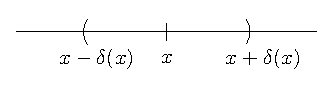
\includegraphics[width=0.35\textwidth]{20_1.eps}
		\caption{Окрестность зависит от точки $x$.}
		\label{20_1}
	\end{figure}
	Окрестности $\MU_{\frac{\delta(x)}{2}}(x)$ - покрывают $K$, когда $x$ пробегает всё $K$.
	\begin{figure}[H]
		\centering
		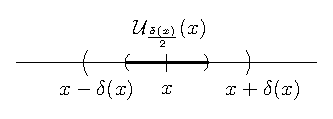
\includegraphics[width=0.35\textwidth]{20_2.eps}
		\caption{Окрестность $\MU_{\frac{\delta(x)}{2}}(x)$.}
		\label{20_2}
	\end{figure}
	Так как $K$ это компакт, то можно выделить конечное подпокрытие: $\exists \, \MU_{\frac{\delta(x_1)}{2}}(x_1), \dotsc , \MU_{\frac{\delta(x_N)}{2}}(x_N)$ - покрытие $K$. Возьмем $\delta = \min\big\{\frac{\delta(x_1)}{2}, \dotsc,\frac{\delta(x_N)}{2} \big\}$. Пусть $|x-y| < \delta$, так как $x,y \in K \Rightarrow \exists \, \MU_{\frac{\delta(x_k)}{2}}(x_k) \ni x$
	\begin{figure}[H]
		\centering
		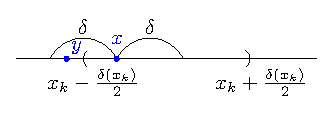
\includegraphics[width=0.35\textwidth]{20_3.eps}
		\caption{$|x-y| < \delta$.}
		\label{20_3}
	\end{figure}
	Поскольку $\delta \leq \frac{\delta(x_k)}{2}$, то получается что $x,y \in \MU_{\delta(x_k)}(x_k)$.
	\begin{figure}[H]
		\centering
		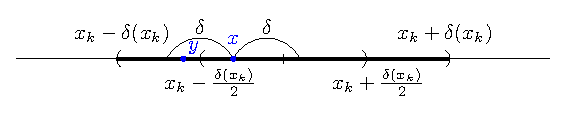
\includegraphics[width=0.65\textwidth]{20_4.eps}
		\caption{$x,y \in \MU_{\delta(x_k)}(x_k)$.}
		\label{20_4}
	\end{figure}
	Поскольку $x,y \in \MU_{\delta(x_k)}(x_k) \Rightarrow |f(x) - f(y)| < \VE$.
	
\end{proof}

Посмотрим на определение равномерной непрерывности и попробуем записать его в терминах колебания функций. 

Пусть $f \colon \MR \to \MR$, рассматриваем непрерывность и равномерную непрерывность на всей $\MR$.

\uline{\textbf{Непрерывность}}: $\forall a \in \MR, \, \lim\limits_{\delta \to 0+}\omega(f,\MU_\delta(a)) = 0$;

\uline{\textbf{Равномерная непрерывность}}: $\lim\limits_{\delta \to 0+}\sup\limits_{a}\omega(f,\MU_\delta(a)) = 0$;

По определению равномерной непрерывности $\forall \VE >0, \exists \, \delta >0 \colon \forall x,y \in D, \, |x-y| < \delta \Rightarrow$ \\
$\Rightarrow |f(x)-f(y)| < \VE \Rightarrow \omega(f,\MU_\frac{\delta}{2}(a)) < \VE$ и это не будет зависеть от $a \Rightarrow$ это сразу для всех $a \Rightarrow$\\ $\Rightarrow \sup\limits_{a}\omega(f,\MU_\frac{\delta}{2}(a)) < \VE$.

\begin{figure}[H]
	\centering
	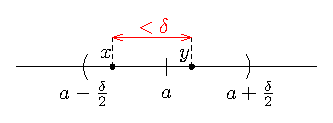
\includegraphics[width=0.35\textwidth]{20_5.eps}
	\caption{Равномерная непрерывность в терминах колебания функции.}
	\label{20_5}
\end{figure}

Можно и в обратную сторону, пусть $\lim\limits_{\delta \to 0+}\sup\limits_{a}\omega(f,\MU_\delta(a)) = 0 \Rightarrow \forall \VE > 0, \exists \, \delta > 0 \colon \sup\limits_{a}\omega(f,\MU_\delta(a)) < \VE \Rightarrow$ возьмем две точки $x,y \in D \colon |x-y| < \delta \Rightarrow$ возьмем середину и будем смотреть колебания функции на окрестности радиуса $\delta$. На всякой такой окрестности, колебания функции будут $<\VE \Rightarrow$ равномерно непрерывна.

В равномерной непрерывности в терминах колебаний записано, что предел приближается к $0$ одновременно во всех точках $a$.

\newpage

\section*{Сходимость функций}

Пусть задана последовательность функций $f_n \colon D \to \MR$.
\begin{defn}
	Последовательность $f_n$ \uwave{сходится к $f$ поточечно}, если $\forall x \in D, \, \lim\limits_{n \to \infty}f_n(x) =f(x)$.
\end{defn}

\begin{defn}
	Последовательность $f_n$ \uwave{сходится к $f$ равномерно на $D$}, если $\lim\limits_{n \to \infty}\sup\limits_{D}|f_n(x) - f(x)| = 0$.
\end{defn}

\uline{\textbf{Поточечная сходимость}}: $\forall x, \, \forall \VE >0, \exists \, N \colon \forall n > N, \, |f_n(x) - f(x)| < \VE$.

\uline{\textbf{Равномерная сходимость}}: $\forall \VE >0, \exists \, N \colon \forall n > N, \, \sup\limits_D|f_n(x) - f(x)| < \VE \Leftrightarrow \forall x \in D, \, |f_n(x) - f(x)| < \VE$, то есть $\forall \VE >0, \exists \, N \colon \forall n > N, \, \forall x \in D, \, |f_n(x) - f(x)| < \VE$.

\textbf{Пример}: $D = [0,1]$, последовательность функций $f_n$ имеют следующий вид:
\begin{figure}[H]
	\centering
	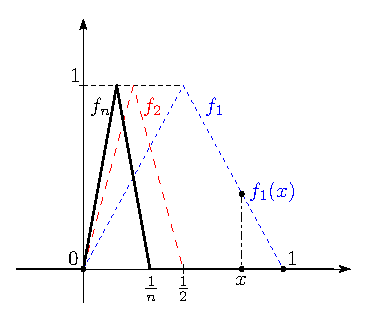
\includegraphics[width=0.35\textwidth]{20_6.eps}
	\caption{Пример поточечной сходимости функций.}
	\label{20_6}
\end{figure}

Рассмотрим точку $x$, сначала функция $f_1$ равна какому-то значению в этой точке, затем значения следующих функций равны $0$ в этой точке $\Rightarrow f_n(x) \to 0$. Таким образом, поточечно, в каждой точке $x$ последовательность $f_n(x)$ стремится к $0$.

Будет ли эта сходимость равномерной? $\sup\limits_{D}|f_n(x) - 0| = 1 \nrightarrow 0$. Если бы равномерно сходилась, то можно было бы указать номер, после которого все значения были бы маленькие. А здесь такой номер указать  невозможно.

\textbf{Пример}: $f_n(x) = \frac{\sin{x}}{n}, \, D = \MR, \, f_n(x) \to 0, \, |f_n(x)| \leq \frac{1}{n} \Rightarrow \sup\limits_{D}|f_n(x)| \leq \frac{1}{n} \to 0 \Rightarrow$ есть равномерная сходимость.

Какие свойства сохраняются при приближении известными функциями неизвестной? В том числе интересуют непрерывность. При поточечной сходимости свойство непрерывности исчезнет, но не совсем, а при равномерной сходимости, непрерывность обязательно сохранится.

\textbf{Пример}: $D = [0,1]$, последовательность функций $f_n$ имеют следующий вид:
\begin{figure}[H]
	\centering
	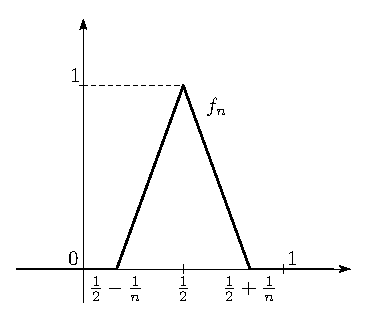
\includegraphics[width=0.35\textwidth]{20_7.eps}
	\caption{Исчезновение непрерывности, при поточечной сходимости функций.}
	\label{20_7}
\end{figure}
Такая последовательность сходится поточечно к функции следующего вида: \\
$f_n(x) \to 0, \, x \neq \frac{1}{2}$ и $f_n(x) \to 1, \, x = \frac{1}{2}$.
Более того, данная сходимость не была равномерной.

Может ли последовательность непрерывных функций сходится к функции Дирихле? Нет и для этого есть следующая теорема.

\begin{theorem}
	Пусть $f_n$ - непрерывна на $\MR$ и поточечно сходится к $f(x) \colon \forall x \in \MR, \, f_n(x) \to f(x)$. Тогда $\exists \, x_0 \in \MR \colon f$ - непрерывна в точке $x_0$.
\end{theorem}
\begin{rem}
	В каждом интервале найдется такая точка. Данное доказательство можно проделать для любого интервала, поэтому в каждом интервале будет точка непрерывности.
\end{rem}

\uline{\textbf{Идея}}: Доказываем от противного, если функция $f$ не является непрерывной в точке $x_0 \Rightarrow$ она всюду разрывна $\Rightarrow$ у нее есть точки в которых колебания положительны, то есть рядом с которыми функция ведет себя как функция Дирихле. Так как $f_n$ сходится поточечно, то в каждом интервале найдется интервал, где $f_n$ будет ее хорошо приближать (лучше, чем колебания функции).

С одной стороны $f$ скачет, с другой стороны не отличается от функций у которых колебания $= 0 \Rightarrow$ так не может быть, противоречие.


\end{document}